\documentclass{article}
\usepackage[utf8]{inputenc}
\usepackage[T1]{fontenc}
\usepackage{graphicx}
\usepackage{hyperref}
\usepackage{geometry}
\geometry{margin=1in}

\title{THOMISM}
\date{Encyclopaedia Britannica (1771)}

\begin{document}
\maketitle

\section*{Historical source}
\textbf{Entry ID:} \texttt{entry-thomism-1614} \\
\textbf{Volume ID:} 144133903 \\
\textbf{Character Count:} 632

\subsection*{Extracted Text}
THOMISM, the doctrine of St Thomas Aquinat, and his followers the Thomas, clearly with regard to predellination and grace. There is some doubts what the true ge mine thomlim is, but there are authors who diflingwith the thomall of St Thomas from that of the dominicians. Other agents make themomin so more than a kind of inni-fenim olugted: bat janfenim, it is known, has been condemned by the repys, which give thomlim never was: in effect, the writings of diverse Lesenc, who were appointed by their order to lay down and defend, before the baby five, the depunts of their School, have face been reported the role of pure thomlim.



\section*{Source record}
\begin{itemize}
\item \textbf{Dataset:} \texttt{NationalLibraryOfScotland/encyclopaedia\_britannica\_illustrated}
\item \textbf{Dataset Revision:} \texttt{309f765b1ecc83e0a7f7762e44b4a927a7555443}
\item \textbf{Page ID:} \texttt{britannica:309f765b1ecc83e0a7f7762e44b4a927a7555443:train:1614} \\
  \textbf{Filename:} \texttt{page-1614-ea352b487d65.jpg} \\
  \textbf{Row Index:} 1614 \\
  \textbf{SHA256:} \texttt{ea352b487d650c71...}
\end{itemize}

\begin{figure}[h]
\centering
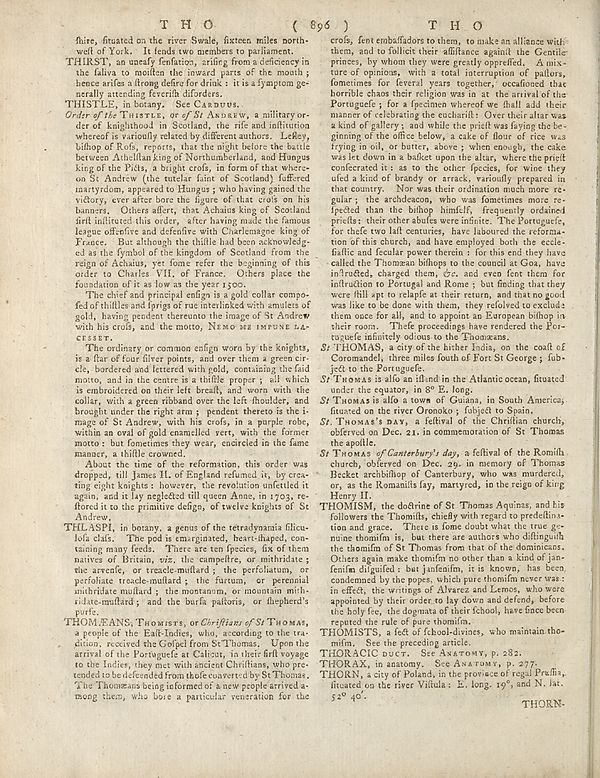
\includegraphics[width=0.85\textwidth]{../scans/page-1614-ea352b487d65.jpg}
\caption*{Source scan: \texttt{page-1614-ea352b487d65.jpg}}
\end{figure}

\end{document}
